\documentclass[11pt]{scrartcl}
\usepackage[scale=1.5]{ccicons}
\usepackage[notextcomp]{kpfonts} 
\usepackage[margin=1.0in]{geometry}
\usepackage{amsthm,amssymb,amsmath}
\usepackage{graphicx}
\usepackage{enumitem}
\usepackage{bm}
\usepackage{tabu}
\usepackage{mathtools}
\usepackage{tikz}
\usepackage{tikz-3dplot}
\usepackage{xcolor}
\usepackage{colortbl}
\usepackage{wasysym}
\usepackage{wrapfig}
\usepackage{tabularx}


\newcolumntype{C}{>{\raggedright\arraybackslash $}X<{$}}



\usepackage{color}
\definecolor{darkblue}{rgb}{0, 0, .6}
\definecolor{grey}{rgb}{.7, .7, .7}
\usepackage[breaklinks]{hyperref}
\hypersetup{
	colorlinks=true,
	linkcolor=darkblue,
	anchorcolor=darkblue,
	citecolor=darkblue,
	pagecolor=darkblue,
	urlcolor=darkblue,
	pdftitle={},
	pdfauthor={}
}
\usepackage{fancyhdr}
\thispagestyle{fancy}
\lhead{}
\chead{Math 112 Section 006/010 Laird}
\rhead{}
%\lfoot{}%\scriptsize This work is licensed under the \href{http://creativecommons.org/licenses/by-sa/3.0/us/}{Creative Commons Attribution-Share Alike 3.0 License}.} 
%\cfoot{}
%\rfoot{\ccbysa}
\renewcommand{\headrulewidth}{.4pt}
%\renewcommand{\footrulewidth}{.4pt}

\theoremstyle{definition}
\newtheorem{theorem}{Theorem}
\newtheorem*{theorem*}{Theorem}
\newtheorem{acknowledgement}[theorem]{Acknowledgement}
\newtheorem{algorithm}[theorem]{Algorithm}
\newtheorem{axiom}[theorem]{Axiom}
\newtheorem{case}[theorem]{Case}
\newtheorem{claim}[theorem]{Claim}
\newtheorem*{claim*}{Claim}
\newtheorem{conclusion}[theorem]{Conclusion}
\newtheorem{condition}[theorem]{Condition}
\newtheorem{conjecture}[theorem]{Conjecture}
\newtheorem{corollary}[theorem]{Corollary}
\newtheorem{criterion}[theorem]{Criterion}
\newtheorem{definition}[theorem]{Definition}
\newtheorem{example}[theorem]{Example}
\newtheorem{exercise}[theorem]{Exercise}
\newtheorem{journal}[theorem]{Journal}
\newtheorem{lemma}[theorem]{Lemma}
\newtheorem{notation}[theorem]{Notation}
\newtheorem{problem}[theorem]{Problem}
\newtheorem*{problem*}{Problem}
\newtheorem{proposition}[theorem]{Proposition}
\newtheorem{remark}[theorem]{Remark}
%\newtheorem{solution}[theorem]{Solution}
\newtheorem{summary}[theorem]{Summary}
\newtheorem{skeleton}[theorem]{Skeleton Proof}
\newtheorem{activity}[theorem]{Activity}
\newtheorem{intuitivedef}[theorem]{Intuitive Definition}

\DeclareMathOperator{\spn}{span}
\DeclareMathOperator{\Char}{Characteristic}
\DeclareMathOperator{\Aut}{Aut}
\DeclareMathOperator{\stab}{Stab}
\DeclareMathOperator{\Stab}{Stab}
\DeclareMathOperator{\orb}{\mathcal{O}}
\DeclareMathOperator{\lcm}{lcm}
\DeclareMathOperator{\gl}{GL}
\DeclareMathOperator{\Ker}{Ker}
\DeclareMathOperator{\Z}{\mathbb{Z}}
\DeclareMathOperator{\C}{\mathbb{C}}
\DeclareMathOperator{\R}{\mathbb{R}}
\DeclareMathOperator{\N}{\mathbb{N}}
\DeclareMathOperator{\Q}{\mathbb{Q}}
\DeclareMathOperator{\A}{\mathbb{A}}
\DeclareMathOperator{\Gal}{Gal}
\DeclareMathOperator{\PS}{\mathcal{P}}
\DeclareMathOperator{\acc}{acc}
\DeclareMathOperator{\mstar}{\mu^\ast}
\DeclareMathOperator{\M}{\mathcal{M}}
\DeclareMathOperator{\el}{\mathcal{L}}
\DeclareMathOperator{\dm}{d\mu}


\newenvironment{solution}{\begin{proof}[Solution]}{\end{proof}}
\newcommand{\comment}[1]{%
  \text{\phantom{(#1)}} \tag{#1}
}

\pagenumbering{gobble}

%Useful for cut and paste
%\begin{enumerate}[label=\rm{(\alph*)}]

\begin{document}

\newpage
\thispagestyle{fancy}

%\noindent
%\textit{Directions: Work individually in pencil until time is called. Then discuss with your nearest neighbor and make corrections in pen. Each person should show their work and turn in their paper. Any work done on the calculator should be indicated with a quick sketch or a description of the process used.}

\textit{Directions: Using your graphing calculator fill out the following table with your group}

\vspace{0cm}

%\noindent
%For the function $g(x)=\frac{3x-2}{x+4}$,
%\begin{enumerate}
%	\item Find the domain of $g(x)$. 
%	\vspace{6.5cm}
%	\item For what values of $x$ is $f(x)=0$?
%\end{enumerate}



%\begin{center}
%	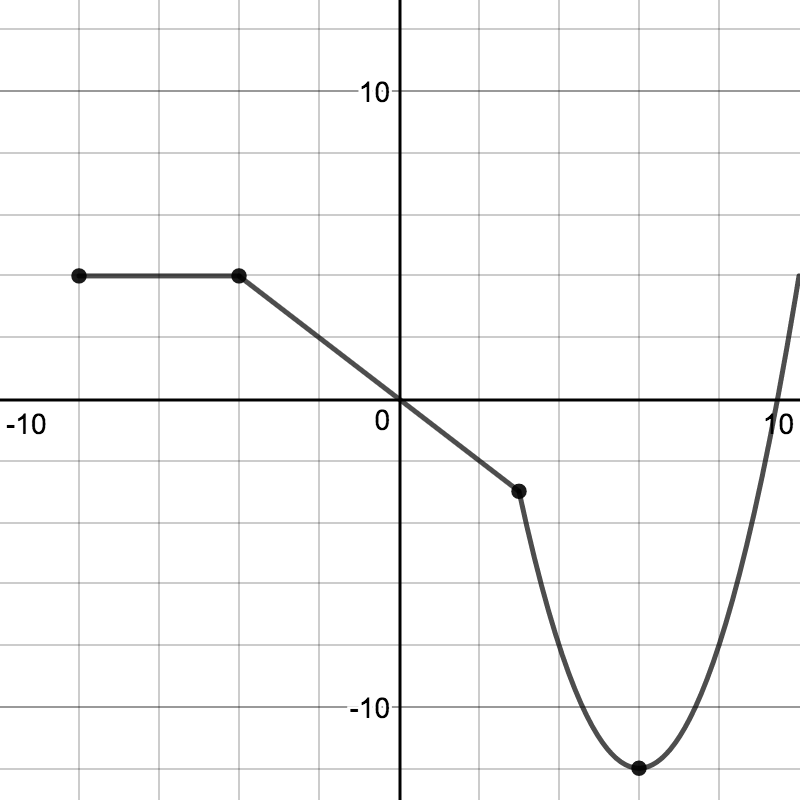
\includegraphics[scale=0.3]{conceptcheck3}
%\end{center}
%
%\noindent
%Please identify all of the following features of the graph:
%\begin{enumerate}
%	\item Domain:
%	\item Range:
%	\item Interval(s) on which the function is increasing:
%	\item Interval(s) on which the function is decreasing:
%	\item Interval(s) on which the function is negative:
%	\item Interval(s) on which the function is positive:
%\end{enumerate}


%A business bought a machine for \$35,000. After 4 years the machine is valued at \$15,000. Assume the value of the machine depreciates linearly.
%\begin{enumerate}
%	\item Express the value of the machine as a function of time in years. \vspace{4.5cm}
%	\item What is the slope of this linear function, and what does it tell you in practical terms? (include units) \vspace{4.5cm}
%	\item What is the $x$-intercept of this function and what does it tell you in practical terms?
%\end{enumerate}


%\noindent
%A certain state uses the following information to determine income taxes. 
%\begin{itemize}
%	\item Incomes between \$0 and \$50,000 are assessed a 9\% tax
%	\item Incomes over \$50,000 are assessed a 9\% tax on the first \$50,000 and a 12\% tax on the income over \$50,000
%\end{itemize}
%
%\noindent 
%Use this information to answer the next three questions. \vspace{1cm}
%
%\begin{enumerate}
%	\item Determine a piecewise function that represents the tax in terms of income $x$.
%	\vspace{5cm}
%	\item If a person had a salary of \$70,000, how much tax would they owe?
%\end{enumerate}

%\noindent
%\begin{enumerate}
%	\item Graph the following function:
%			\[ f(x) = \begin{cases}
% 					x+3 & \text{if } x \leq -1\\
% 					4 & \text{if } x > -1
% 					\end{cases} \]
% 			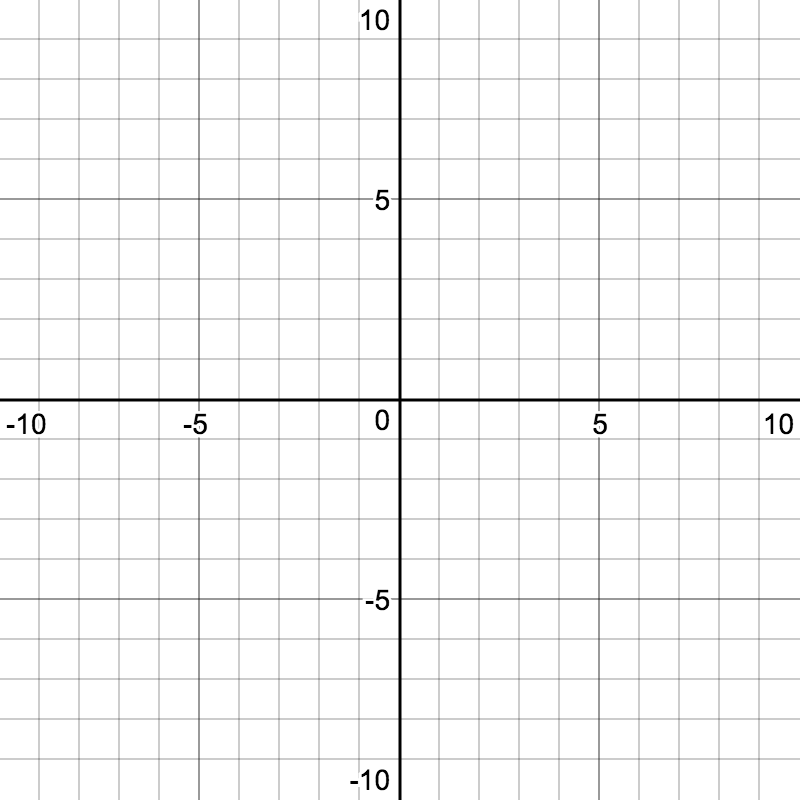
\includegraphics[scale=0.2]{grid}		
% 	
% 	\vspace{0.2cm}
%
%	\item Determine an equation for the following piecewise function:\\
%	
%	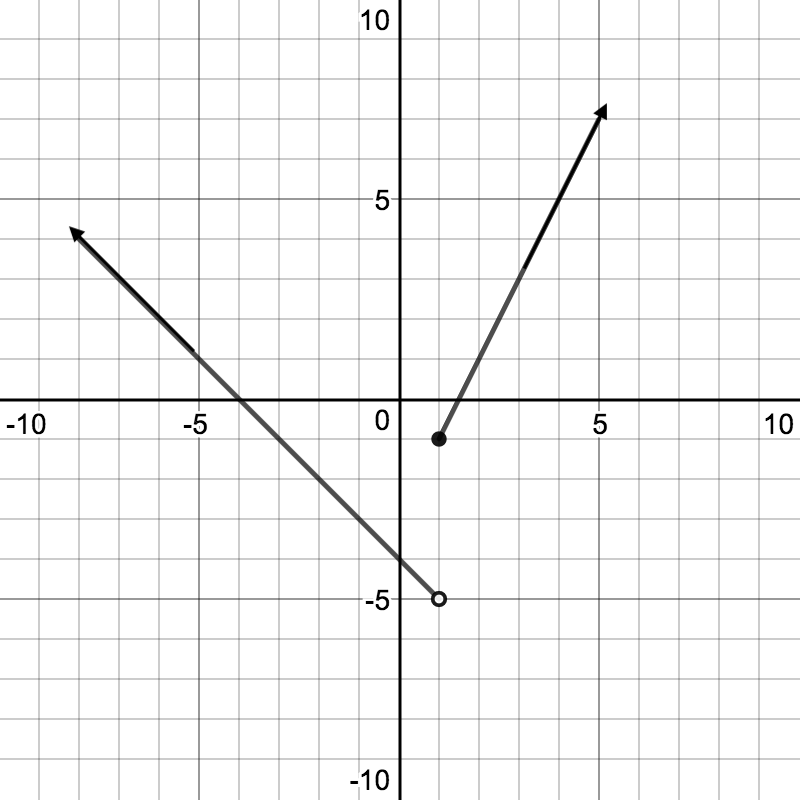
\includegraphics[scale=0.2]{Piecewise2}
%\end{enumerate}

%\noindent
%\begin{enumerate}
%	\item The graph of $y=f(x)$ is given below. On the same set of axes, sketch the graph of $y=3f(x+2)-3$. \\ 
%		\begin{center}
%			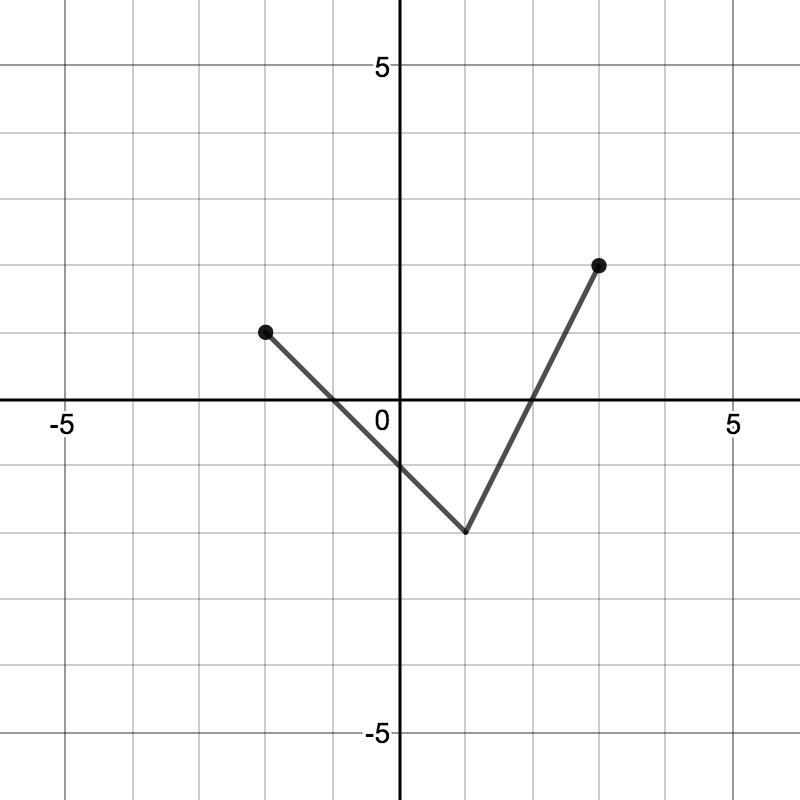
\includegraphics[scale=0.25]{transformations1} 
%		\end{center}
%		\vspace{1cm}
%		State the domain and the range:\\ \[ \textbf{Domain: \underline{\hspace{4cm}}} \] \vspace{1.5cm} \[ \textbf{ \hspace{0.5em}Range: \underline{\hspace{4cm}}} \] 
%
%\end{enumerate}

%%%%%%%%%%%%%%%%%%%%%%%%% Day 20 Print Offs %%%%%%%%%%%%%%%%%%%%%%%%
\begin{tabularx}{\textwidth}{@{\rule[-10ex]{0pt}{7ex}}|*{6}{C|}}
\hline
 & \text{Degree} & \text{Leading Term} & \text{Graph} & \text{Zeros} & \text{Factored}  \\
\hline
y=x &  &  &  &  &    \\
\hline
y=x^2 &  &  &  &  &    \\
\hline
y=x^3 &  &  &  &  &    \\
\hline
y=x^4 &  &  &  &  &    \\
\hline
y=x^5 &  &  &  &  &    \\
\hline
y=-\frac{1}{5}x^4-\frac{1}{5}x^3+\frac{8}{5}x^2+\frac{12}{5}x &  &  &  &  &    \\
\hline
y=x^3-9x^2+27x-27 &  &  &  &  &    \\
\hline
y=x^4-7x^3+9x^2+27x-54 &  &  &  &  &    \\
\hline
y=-x^3-3x^2+5x-7 &  &  &  &  &    \\
\hline
y=-\frac{1}{2}(x-3)^2(x-5) &  &  &  &  &    \\
\hline
    \end{tabularx}

\end{document}
























